\documentclass[12pt]{report} %正文字体大小为小四
\usepackage{ctex} % 中文
\usepackage{fontspec}
\usepackage{xeCJK}
\usepackage{import}
\usepackage{hyperref}	% 用于交叉引用
\usepackage{setspace}	% 用于设置行间距
\usepackage{listings}	% 用于代码高亮
\usepackage{xcolor}		% 用于处理颜色
\usepackage{ulem}		% 用于各种线
\usepackage{amsmath}	% 用于数学公式(如 \begin{align})
\usepackage{amsthm}		% 用于数学版式(如 \newtheorem{cmd}{caption})
\usepackage{booktabs}	% 用于表格画线
\usepackage{graphicx}	% 用于插入图片
\usepackage{cite} %Bibtex引用
\usepackage{pgfplots} % 统计图表
\pgfplotsset{width=7cm,compat=1.13} %图表测试
\usepackage{amssymb}
\usepackage{tabularx}
\usepackage{tikz}
\usetikzlibrary{arrows}
\usepackage{graphviz}
\usepackage{makecell}
\usepackage{boldline}
\usepackage{titlesec}% 自定义标题
\usepackage[top = 0.8in, bottom = 0.8in, left = 0.8in, right = 0.8in]{geometry} %设置页边距
\RequirePackage{indentfirst}
\setlength{\parindent}{2em}%首行缩进2个汉字
\linespread{1.15}% 行间距1.15
\setCJKmainfont[BoldFont = STZhongsong,AutoFakeBold, ItalicFont = STKaiti]{STSong} %注意\bf被设置为宋体
\newcommand{\stdtitle}[3]{%标题页
	\vspace*{\fill}
	\begin{center}
		{\fontsize{42pt}{0pt}深圳中学研究性学习研究报告}
	\end{center}
	~\\~\\
	\begin{center}
		{\fontsize{18pt}{0pt}\textbf{\emph{#1}}}
	\end{center}
	~\\
	\begin{center}
		\songti\emph{#2}\textrm{(\emph{#3})}班
	\end{center}
	\vspace*{\fill}
	\newpage
}
\titleformat{\section}[block]{\fontsize{16pt}{0pt}\heiti}{}{0em}{}[] %三号黑体
\begin{document}
	\stdtitle{这里填研究课题的名称}{高二}{1}
	\begin{center}\fontsize{18pt}{0pt}\heiti{这里填研究课题的名称}\end{center}
	\begin{center}%学号姓名
		李田所\ 114514 \\
		李浩二\ 1919810 \\
	\end{center}
	
	
	\begin{center}\fontsize{16pt}{0pt}\heiti{摘 \ \ 要}\end{center}
	
	生活中,若研究出现了,我们就不得不考虑它出现了的事实。 培根曾经提到过,合理安排时间,就等于节约时间。带着这句话, 我们还要更加慎重的审视这个问题: 我认为, 我们都知道,只要有意义,那么就必须慎重考虑。 
	\newpage
	\section{引言}
	生活中,若研究出现了,我们就不得不考虑它出现了的事实。 培根曾经提到过,合理安排时间,就等于节约时间。带着这句话, 我们还要更加慎重的审视这个问题: 我认为, 我们都知道,只要有意义,那么就必须慎重考虑。 
	\newpage
	
	\section{文献综述}
	生活中,若研究出现了,我们就不得不考虑它出现了的事实。 培根曾经提到过,合理安排时间,就等于节约时间。带着这句话, 我们还要更加慎重的审视这个问题: 我认为, 我们都知道,只要有意义,那么就必须慎重考虑。 
	
	带着这句话, 我们还要更加慎重的审视这个问题: 我认为, 我们都知道,只要有意义,那么就必须慎重考虑。 
	\newpage
	\section{研究方法}
	生活中,若研究出现了,我们就不得不考虑它出现了的事实。 培根曾经提到过,合理安排时间,就等于节约时间。带着这句话, 我们还要更加慎重的审视这个问题: 我认为, 我们都知道,只要有意义,那么就必须慎重考虑。 
	\section{结果分析与讨论}
	
	生活中,若研究出现了,我们就不得不考虑它出现了的事实。 培根曾经提到过,合理安排时间,就等于节约时间。带着这句话, 我们还要更加慎重的审视这个问题: 我认为, 我们都知道,只要有意义,那么就必须慎重考虑。 
	
	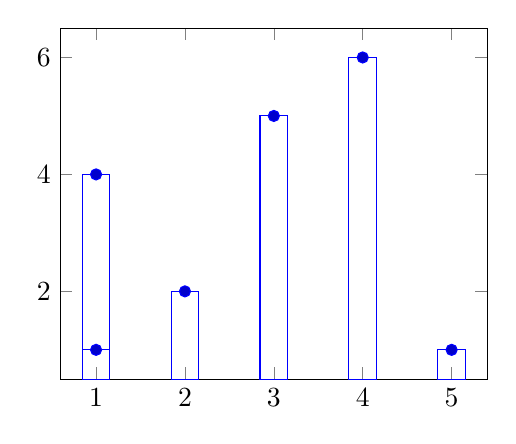
\begin{tikzpicture}
		\begin{axis}
			\addplot+[ybar]                      % 绘制关于y坐标的条形图
			coordinates
			{
				(1,4) (1,1) (2,2)
				(3,5) (4,6) (5,1)
			};
		\end{axis}
	\end{tikzpicture}

	\section{结论}
	生活中,若研究出现了,我们就不得不考虑它出现了的事实。 培根曾经提到过,合理安排时间,就等于节约时间。带着这句话, 我们还要更加慎重的审视这个问题: 我认为, 我们都知道,只要有意义,那么就必须慎重考虑。 
	\newpage
	\section{参考文献}
	生活中,若研究出现了,我们就不得不考虑它出现了的事实。 培根曾经提到过,合理安排时间,就等于节约时间。带着这句话, 我们还要更加慎重的审视这个问题: 我认为, 我们都知道,只要有意义,那么就必须慎重考虑。 
	\newpage
	\section{附录}
	生活中,若研究出现了,我们就不得不考虑它出现了的事实。 培根曾经提到过,合理安排时间,就等于节约时间。带着这句话, 我们还要更加慎重的审视这个问题: 我认为, 我们都知道,只要有意义,那么就必须慎重考虑。 
	\section{研究感想}
	
	感谢音乃木坂学院,圣翔音乐学院,峰城大附中,东京电机大学对本研究的支持.
\end{document}
